\documentclass{standalone}
\usepackage{tikz}
\usetikzlibrary{shapes, arrows.meta, positioning}

\begin{document}
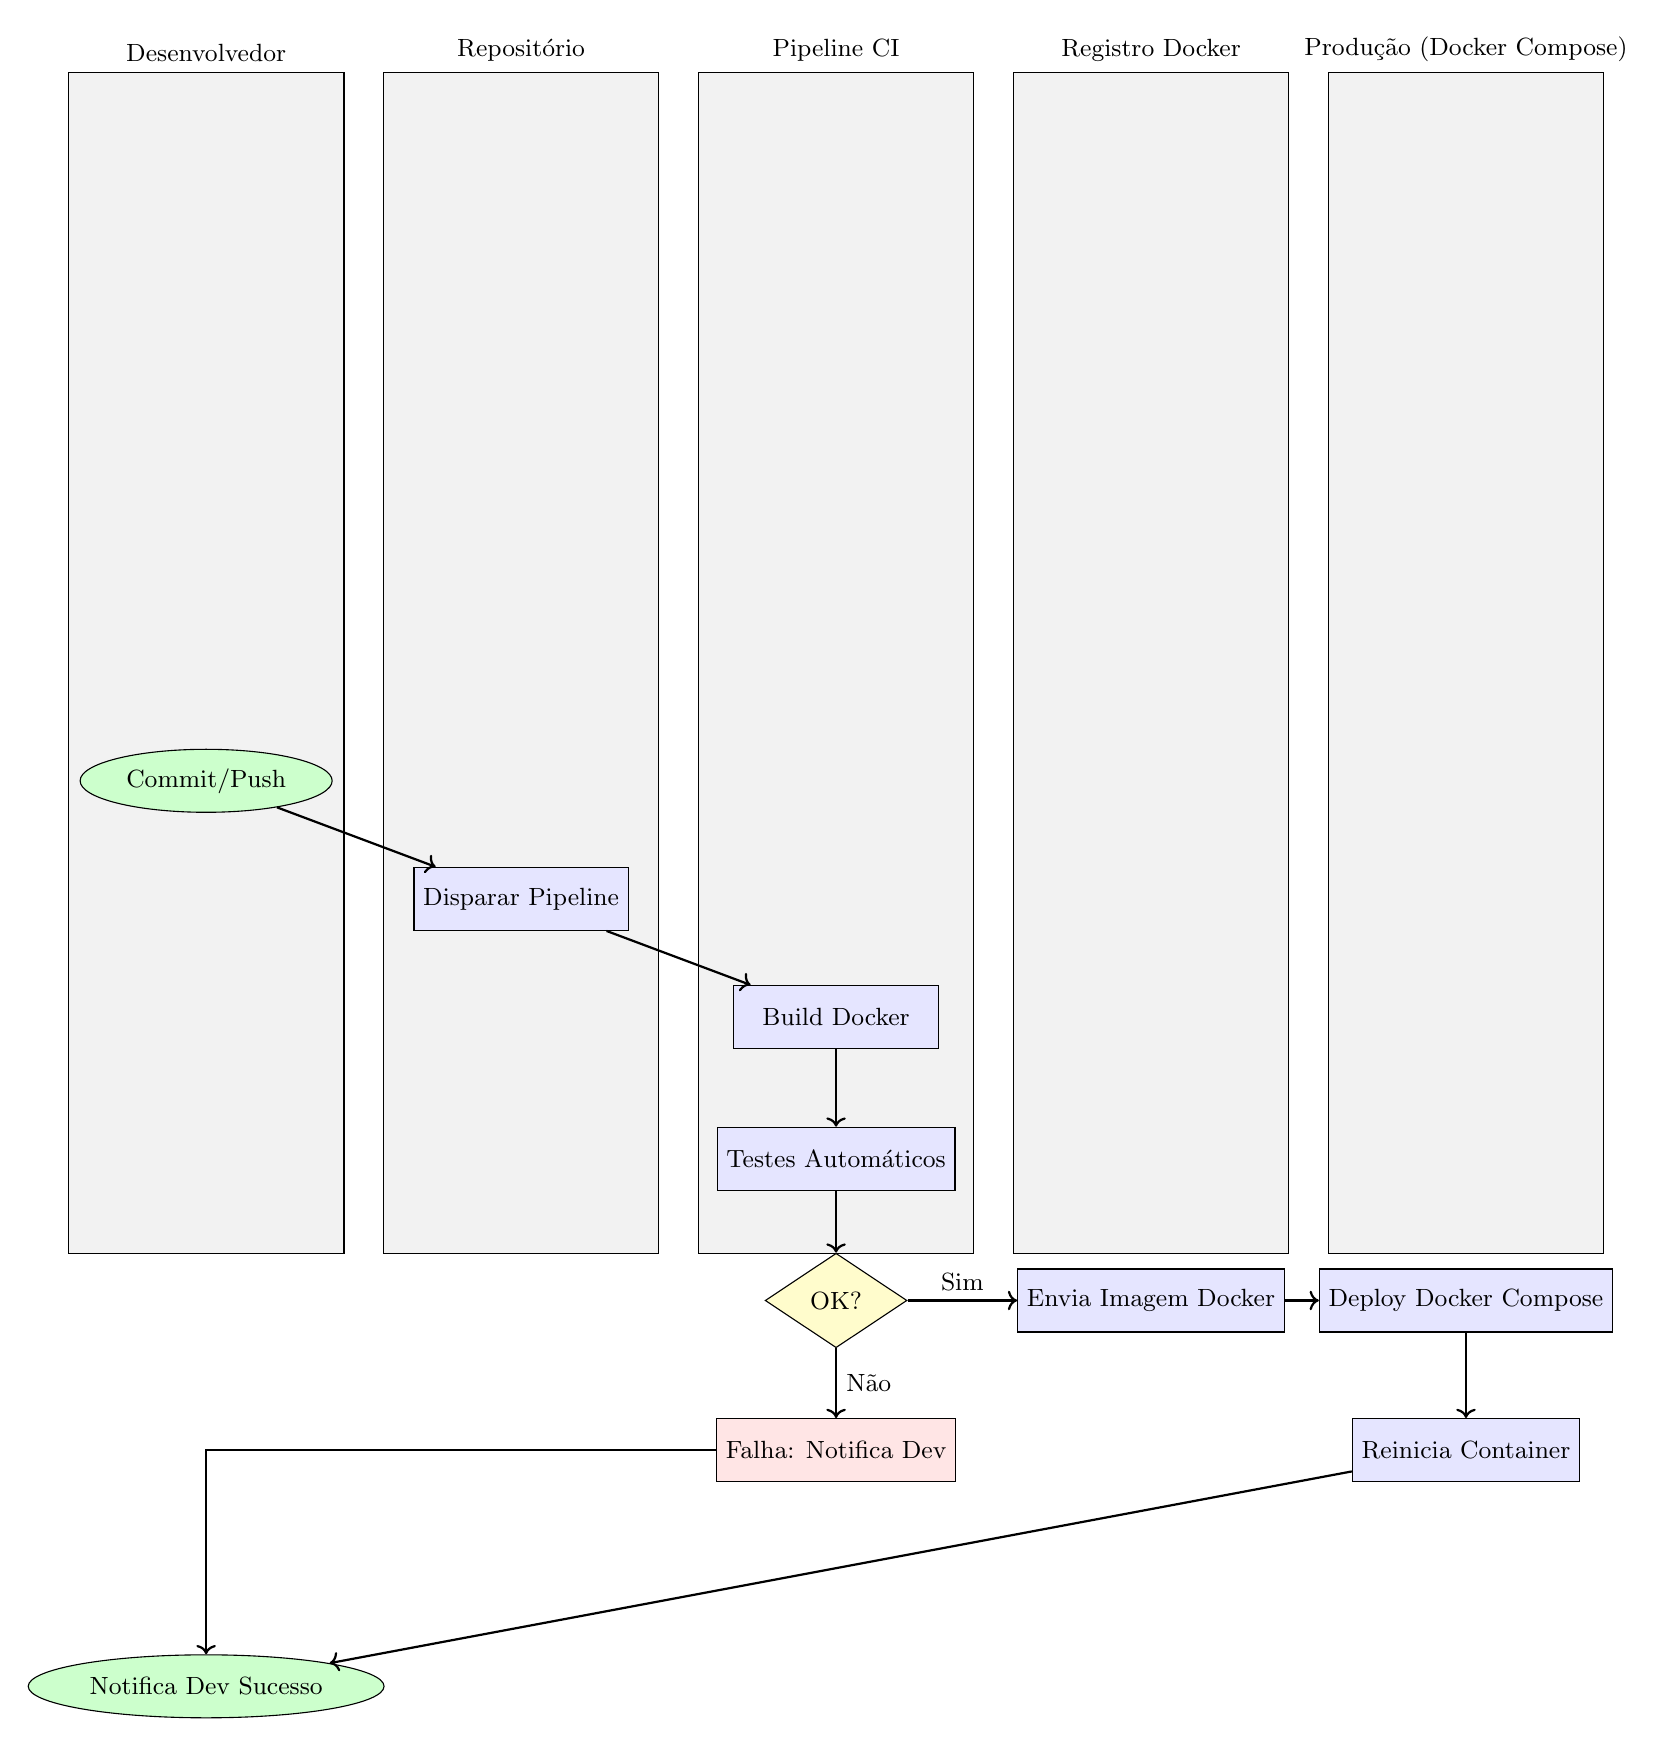
\begin{tikzpicture}[node distance=1.8cm, every node/.style={font=\small},
  swimlane/.style={rectangle, draw, minimum width=3.5cm, minimum height=15cm, fill=gray!10},
  event/.style={ellipse, draw, fill=green!20, minimum width=2.6cm, minimum height=0.8cm},
  task/.style={rectangle, draw, fill=blue!10, minimum width=2.6cm, minimum height=0.8cm},
  gateway/.style={diamond, draw, fill=yellow!20, aspect=2, minimum width=1.2cm, minimum height=1.2cm},
  notify/.style={rectangle, draw, fill=red!10, minimum width=2.6cm, minimum height=0.8cm}
]
% Swimlanes
\node[swimlane, label=above:{Desenvolvedor}] (dev) at (0,0) {};
\node[swimlane, label=above:{Repositório}] (repo) at (4,0) {};
\node[swimlane, label=above:{Pipeline CI}] (ci) at (8,0) {};
\node[swimlane, label=above:{Registro Docker}] (reg) at (12,0) {};
\node[swimlane, label=above:{Produção (Docker Compose)}] (prod) at (16,0) {};
% Eventos e tarefas (alinhados verticalmente nas swimlanes)
\node[event] (start) at (0,-1.5) {Commit/Push};
\node[task] (trigger) at (4,-3) {Disparar Pipeline};
\node[task] (build) at (8,-4.5) {Build Docker};
\node[task] (test) at (8,-6.3) {Testes Automáticos};
\node[gateway] (gw) at (8,-8.1) {OK?};
\node[notify] (fail) at (8,-10) {Falha: Notifica Dev};
\node[task] (pushimg) at (12,-8.1) {Envia Imagem Docker};
\node[task] (deploy) at (16,-8.1) {Deploy Docker Compose};
\node[task] (restart) at (16,-10) {Reinicia Container};
\node[event] (success) at (0,-13) {Notifica Dev Sucesso};
% Fluxos
\draw[->, thick] (start) -- (trigger);
\draw[->, thick] (trigger) -- (build);
\draw[->, thick] (build) -- (test);
\draw[->, thick] (test) -- (gw);
\draw[->, thick] (gw) -- node[right]{Não} (fail);
\draw[->, thick] (gw) -- node[above]{Sim} (pushimg);
\draw[->, thick] (pushimg) -- (deploy);
\draw[->, thick] (deploy) -- (restart);
\draw[->, thick] (restart) -- (success);
% Notificações
\draw[->, thick] (fail) -- ++(-8,0) -- (success);
\end{tikzpicture}
\end{document}
